% Metódy inžinierskej práce

\documentclass[10pt,twocolumn,slovak,a4paper]{article}

\usepackage[slovak]{babel}
%\usepackage[T1]{fontenc}
\usepackage[IL2]{fontenc} % lepšia sadzba písmena Ľ než v T1
\usepackage[utf8]{inputenc}
\usepackage{graphicx}
\graphicspath{ {C:/FIIT/MIP/CV3/} }
\usepackage{url} % príkaz \url na formátovanie URL
\usepackage{hyperref} % odkazy v texte budú aktívne (pri niektorých triedach dokumentov spôsobuje posun textu)

\usepackage{cite}
%\usepackage{times}

\pagestyle{headings}

\title{Názov\thanks{Semestrálny projekt v predmete Metódy inžinierskej práce, ak. rok 2015/16, vedenie: Meno Priezvisko}} % meno a priezvisko vyučujúceho na cvičeniach

\author{Mykola Kornilov\\[2pt]
	{\small Slovenská technická univerzita v Bratislave}\\
	{\small Fakulta informatiky a informačných technológií}\\
	{\small \texttt{xkornilov@stuba.sk}}
	}

\date{\small 10. oktobra 2026} % upravte



\begin{document}

\maketitle

\begin{abstract}
\ldots
\end{abstract}

\section{Úvod}


\section{Nejaká časť} \label{nejaka}


\begin{figure*}[t]
  \centering
  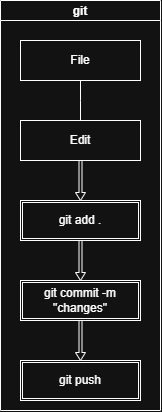
\includegraphics[width=0.25\textwidth]{diagram1}
  \hfill
  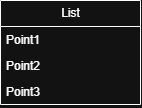
\includegraphics[width=0.25\textwidth]{diagram2}
  \caption{Dva diagramy vedla seba.}
\end{figure*}


\begin{figure*}[t]
  \centering
  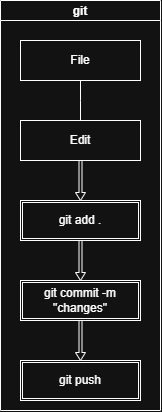
\includegraphics[width=\textwidth]{diagram1}
  \caption{Obrazok cez obe stlpce.}
\end{figure*}

\bibliography{literatura}
\bibliographystyle{plain} % prípadne alpha, abbrv alebo hociktorý iný
\end{document}
